\documentclass{article}

\usepackage{graphicx}

\author{Thomas Dizon}
\title{Implementing a Software Rasterizer in C}

\begin{document}

\maketitle

\begin{figure}[h]
	\centering
	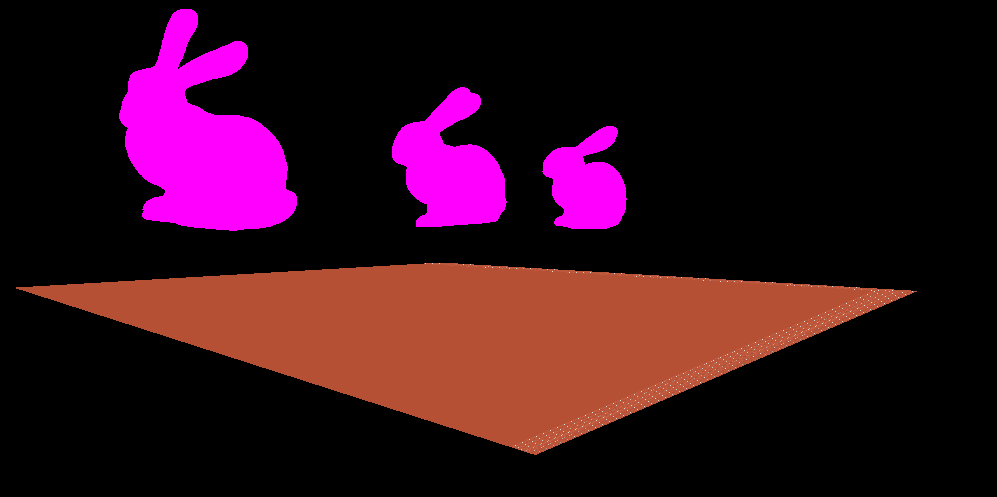
\includegraphics[width=0.6\textwidth]{scene.png}
	\caption{}
\end{figure}

\newpage

\tableofcontents

\newpage

\section{Introduction}

\subsection{Motivation}

\subsection{What is a \textit{Software Rasterizer}?}

\subsection{Why \textit{C}?}


\section{Background}

\subsection{Algorithms}
\subsubsection{Rasterisation}
\subsubsection{Clipping}
\subsubsection{Bresenham Line Drawing}
\subsubsection{Anti-Aliasing}

\subsection{Math Concepts}
\subsubsection{Vectors}
\subsubsection{Matrices}
\subsubsection{Transformations}

\section{System Architecture}

\subsection{Overview}
\subsubsection{System Diagram}
\subsubsection{Project Structure}
\subsubsection{Conventions}

\subsection{Data Design}
\subsubsection{Vectors \& Matrices}
\subsubsection{Primitives: Triangles and Vertices}
\subsubsection{Textures and Materials}
\subsubsection{Framebuffer and Zbuffer}
\subsubsection{Scene, GameObject, Camera, LightObject}

\subsection{Software Design}
\subsubsection{Procedural Programming vs. Object Oriented Programming}
\subsubsection{Graphics Pipeline}
\subsubsection{Scene Management}
\subsubsection{Rendering}
\subsubsection{Shading}

\section{Conclusion \& Future Work}

\subsection{What I learnt}

\subsection{Limitations}

\subsection{A future implementation in C++}


\section{References}

\end{document}

